\documentclass[compress]{beamer}%
\usepackage[utf8]{inputenc}
\usetheme{Warsaw}


\title{Spring}
\subtitle{SoC -- IoC -- DI}

\author{Thomas Duchatelle (duchatelle.thomas@gmail.com)}
\institute{Capgemini, pour Yves Rocher}

\setbeamertemplate{navigation symbols}{} 
\useoutertheme{infolines}
\setbeamertemplate{footline}
{%
  \leavevmode%
  \hbox{\begin{beamercolorbox}[wd=.5\paperwidth,ht=2.5ex,dp=1.125ex,leftskip=.3cm plus1fill,rightskip=.3cm]{author in head/foot}%
    \usebeamerfont{author in head/foot}\insertshortauthor
  \end{beamercolorbox}%
  \begin{beamercolorbox}[wd=.41\paperwidth,ht=2.5ex,dp=1.125ex,leftskip=.3cm,rightskip=.3cm plus1fil]{title in head/foot}%
    \usebeamerfont{title in head/foot}\insertshorttitle 
  \end{beamercolorbox}%
  \begin{beamercolorbox}[wd=.09\paperwidth,ht=2.5ex,dp=1.125ex,leftskip=.3cm plus1fill,rightskip=.3cm]{author in head/foot}%
    \usebeamerfont{author in head/foot}\insertframenumber/\inserttotalframenumber
  \end{beamercolorbox}}%
  \vskip0pt%
}

\AtBeginSection[]{
  \begin{frame}{Sommaire}
  \small \tableofcontents[currentsection, hideothersubsections]
  \end{frame} 
}

\definecolor{fontcolor}{rgb}{0.92,0.92,0.99}
\usepackage{listings}
\lstset{language=Java, numbers=left, tabsize=2, frame=single, breaklines=true,  numberstyle=\tiny\ttfamily,basicstyle=\small, framexleftmargin=5mm, backgroundcolor=\color{fontcolor}, xleftmargin=5mm, basicstyle=\tiny }

\graphicspath{images}

\begin{document}


% Pages de présentations...
\frame{\titlepage}
  
\section*{Plan}
\frame{\tableofcontents[hideallsubsections]}
	
%%%%%%%%%%%%%%%%%%%%%%%%%%%%%%%%%%%%%%%%%
%% SOA
\section{Séparation des préoccupations}

\subsection{Définition}

\begin{frame}{Séparation des préoccupations}
%	\framesubtitle{SoC}
	
	\begin{block}{SoC : Separation of Concerns}
	Pris isolément, chaque problème est plus facile à traiter.
	\end{block}

	\pause
	Découpage de l'application pour isoler les problématiques :
	\begin{itemize}
	\item persistance
	\item services métier
	\item présentation (IHM Web)
	\item appel webservice
	\item ...
	\end{itemize}
	
	\pause
	\begin{block}{Beans}
	Pour chaque nature de problématique : conception de "composants spécialisés", de \emph{briques applicatives}.
	\end{block}
\end{frame}

\subsection{Cas concret}

\begin{frame}{Cas concret}
	\framesubtitle{Embauche d'un nouvel employé}
	
	\begin{exampleblock}{Nouvelle embauche}
	Intégration dans le SI d'un nouvel employé : création de son matricule, email et insertion dans le système des ressources humaines.
	\end{exampleblock}
	
	\pause
	Processus métier pour l'embauche d'un nouveau client :
	\begin{enumerate}[<+->]
		\item un utilisateur autorisé renseigne le nom, prénom et intitulé du poste du nouvel employé
		\item le système génère le matricule de l'employé : identifiant unique
		\item le système génère l'email de l'employé : à partir de son nom et prénom, unique aussi
		\item toutes ces données sont conservées dans le Référentiel Employés
		\item le système informe l'application des Ressources Humaines de la création de nouvel employé
	\end{enumerate}	
	
\end{frame}

\begin{frame}{Méga script !}
	\framesubtitle{Un script PHP suffit}
	
	\begin{itemize}[<+->]
	\item Un tel processus pourrait être écrit en un seul script PHP...\\
	\item Mais :
	\begin{itemize}[<+->]
	\item difficulté d'écrire le script
	\item longueur et lisibilité du script ?
	\item tests de tous les cas
	\end{itemize}
	\end{itemize}
	
\end{frame}

\begin{frame}{Séparation des préoccupations}
	\framesubtitle{Division de la problématique en petites sous problématique}
	
	Proposition de découpage :
	\pause
	\begin{itemize}[<+->]
	\item \emph{IHM} (couche de présentation) : propose une interface intuitive à l'utilisateur afin de récolter les données
	\item \emph{Gestionnaire des Employés} (objet métier) : détient les règles et le processus de création d'un employé
	\item \emph{Générateur de matricules} (objet métier) : détient les règles de génération d'un identifiant unique
	\item \emph{Générateur d'email} (objet métier) : génère un email à partir du nom et prénom.
	\item \emph{DAO Employés} (objet d'accès aux données) : persiste l'employé et détermine si un email est disponible
	\item \emph{Connecteur WS RH} (objet métier) : gère la connexion avec le webservice de l'application des ressources humaines.
	\end{itemize}
	
\end{frame}

\begin{frame}
	\frametitle{Architecture de l'exemple}
	
	\begin{center}	
	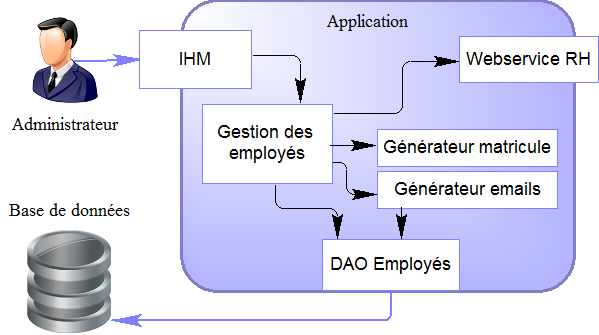
\includegraphics[width=\textwidth]{images/spring_usecase.png}
	\end{center}
\end{frame}
	

\section{Inversion de contrôle}

\subsection{Injection de dépendances}
% les beans ne sont plus responsables de trouver leurs dépendances

\begin{frame}[containsverbatim]{Comment gérer autant debriques applicatives ?}
	\framesubtitle{Approche naïve}
	
	Instanciation des dépendances du bean :
	\begin{lstlisting}
public class EmployeeManager {
	
  private EmployeeNumberGenerator employeeNumberGenerator;		
  
  private EmailGenerator emailGenerator;		
  
  private EmployeeDAO employeeDAO;
		
  public EmployeeManager(Datasource datasource) {
    // Generateur de matricule n'a pas de dependance
    employeeNumberGenerator = new EmployeeNumberGenerator();
			
    employeeDAO = new EmployeeDAO();
    employeeDAO.setDatasource(datasource);// confiruration les datasources !!
			
    emailGenerator = new EmailGenerator();
    emailGenerator.setEmployeeDAO(employeeDAO); // ajout des dependance
  }
}
	\end{lstlisting}
	
\end{frame}

\begin{frame}{Comment gérer autant de \emph{briques applicatives} ?}
	\framesubtitle{Approche naïve}
	
	\begin{alertblock}{Pas de singleton possible}
	Une nouvelle instance d'un bean est créée à chaque fois.
	\end{alertblock}
	
	\pause
	\begin{alertblock}{Couplage fort}
	La dépendance doit connaitre l'implémentation de ses dépendances, ainsi que les dépendances des dépendances (et ainsi de suite) !
	\end{alertblock}
	
\end{frame}

\begin{frame}[containsverbatim]{Comment gérer autant de briques applicatives ?}
	\framesubtitle{Approche par \emph{Factory}}
	
	Utilisation d'une fabrique d'objets
	\begin{lstlisting}
public class EmployeeManager {
	
  private IEmployeeNumberGenerator employeeNumberGenerator = Factory.getEmployeeNumberGenerator();		
  
  private IEmailGenerator emailGenerator = Factory.getEmailGenerator();
}
	\end{lstlisting}
	
	
\end{frame}

\begin{frame}{Comment gérer autant de \emph{briques applicatives} ?}
	\framesubtitle{Approche par \emph{Factory}}

	\begin{exampleblock}{Mutualisation de la création d'objets}
	\begin{itemize}[<+->]
	\item Les méthodes sont réutilisables.
	\item Les implémentations des beans ne sont connues que de la fabrique : utilisation \emph{interfaces}.
	\end{itemize}
	\end{exampleblock}
	
	\pause
	\begin{alertblock}{Couplage toujours important}
	Dépendance vis à vis de la fabrique.
	\end{alertblock}
	
	\pause
	\begin{alertblock}{Configuration}
	Comment faire passer la source de données ? 	
	\begin{itemize}[<+->]
	\item méthode statiquement : peu intuitif et source d'erreurs
	\item argument de la méthode : couplage fort
	\end{itemize}
	\end{alertblock}
% Le code de la fabrique est lourd à écrire...
\end{frame}


\begin{frame}{Comment gérer autant de \emph{briques applicatives} ?}
	\framesubtitle{Approche idéale : injection de dépendances}

	Objectifs de l'approche idéale :
	\begin{itemize}
	\item L'\texttt{EmployeeManager} ne crée pas ses dépendances
	\item Il ne récupère pas ses dépendances d'un tiers
	\end{itemize}
	
	\pause
	Comment ?
	\begin{itemize}
	\item Il va être créé par un composant externe (équivalent d'une fabrique)
	\item Ce composant externe va lui injecter les dépendances dont il a besoin
	\end{itemize}
	
\end{frame}


\begin{frame}{Comment gérer autant de \emph{briques applicatives} ?}
	\framesubtitle{Approche idéale : injection de dépendances}
	
	\begin{block}{Injection de dépendances}
	Le concept d'injection de dépendances est d'instancier un bean, et de lui injecter, par constructeur ou par setter ses dépendances.
	\end{block}	
\end{frame}


\subsection{Gestion de la configuration}
% les beans ne sont plus responsables de leur propre configuration

\begin{frame}{Gestion de la configuration}
	\framesubtitle{Approche naïve}
	
	\begin{block}{Accès direct}
	Chaque bean est responsable de sa configuration : il utilise sa propre méthode et y accède lui même.
	\end{block}
	
	\pause	
	\begin{exampleblock}{Exemple}
	La couche d'accès aux données utilise un "\texttt{ConnectionManager}" qui récupère les sources de données par \emph{JNDI}.
	\end{exampleblock}
	
\end{frame}

\begin{frame}{Exemple de l'approche directe}

	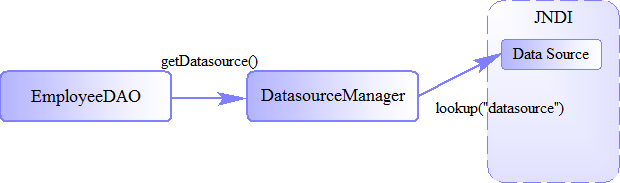
\includegraphics[width=\textwidth]{images/spring_datasource_without.png}
	
	\pause
	Différences sur les environnements :
	\begin{itemize}[<+->]
	\item Sur un serveur d'application \textbf{OK}.
	\item Serveur local : nécessite de paramétrer les sources de données
	\item Tests local (unitaires) : nécessite de forcer la configuration. Lourdeur d'écriture des tests.
	\item En mode standalone (batch) : création d'un "faux" contexte JNDI renseigné à partir d'un autre système de configuration !
	\end{itemize}
	
	
\end{frame}

\begin{frame}{Conclusion de cette première approche}
	
	\begin{alertblock}{Cohérence}
	Aucune gestion globale : cohérence des méthodes entre les beans système. Possible duplications de code et impossibilité de partage d'une même configuration.%exemple : nom d'un serveur cible qui risque d'être dupliqué...
	\end{alertblock}
	
	\pause
	\begin{alertblock}{Couplage fort}
	Aucune flexibilité propre à l'environnement d'exécution n'est permise.
	\end{alertblock}
\end{frame}

\begin{frame}{Gestion de la configuration}
	\framesubtitle{Approche idéale}
	
	\begin{block}{Injection de la configuration}
	La configuration est paramétrée de façon globale (properties, jndi, ...) et est distribuée à tous les beans qui en ont besoin.
	\end{block}
	~\\
	
	\pause	
	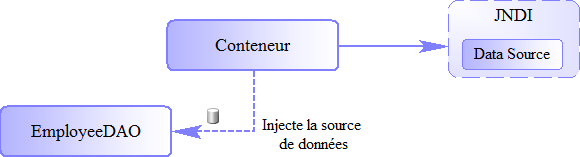
\includegraphics[width=\textwidth]{images/spring_datasource_with.png}
\end{frame}


\subsection{Cycles de vie}
% c'est Spring qui décide quand créer un objet, et quand le détruire.

\begin{frame}{Cycle de vie}

	\begin{block}{Cycle de vie}
	L'instanciation et la destruction des objets sont gérés par le conteneur. Il gère lui même les singletons.
	\end{block}

\end{frame}

\subsection{Bilan}
%% Bilan avec beau graphique de la IoC

\begin{frame}{Inversion de Contrôle}
	\framesubtitle{Association de 3 grands patterns}
	
	\begin{columns}
		\begin{column}{0.5\textwidth}
			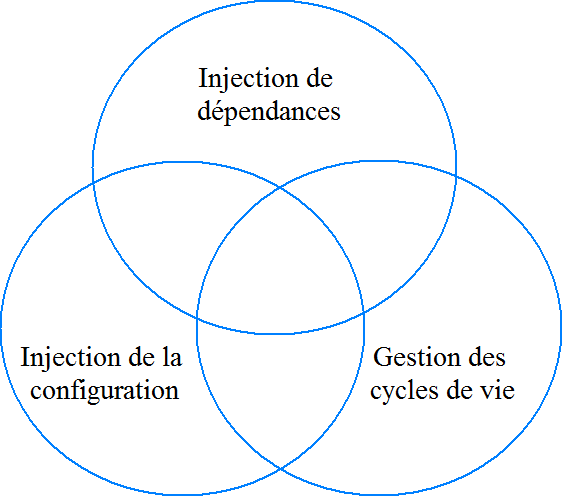
\includegraphics[width=\textwidth]{images/spring_ioc.png}
		\end{column}
		\begin{column}{0.5\textwidth}
			Les 3 grands patterns :
			\begin{itemize}
			\item \textbf{Injection de dépendances}	
			\item \textbf{Injection de la configuration}
			\item \textbf{Gestion des cycles de vie}
			\end{itemize}
		\end{column}
	\end{columns}

\end{frame}


\section{Spring}

\subsection{Définition}
% conteneur léger ? pas d'application, seulement un JAR
% opposition avec les EJB qui demandent un serveur d'applications (Websphère)

% Cartography "IoC et bien autres choses !"

\begin{frame}{Spring = Conteneur léger !}
	\framesubtitle{Définitions ...}
	
	\begin{block}{Conteneur}
	Infrastructure prenant en charge la création d'objets et leurs dépendances : mise en relation d'objets via des fichiers de configuration.
	\end{block}

\end{frame}


\subsection{Configuration}

% XML => déclaration de l'utilisation des annotations
% Création d'un contexte applicatif => uniquement en Java SE


\subsection{Utilisation}
% Déclaration d'un Bean

% Injection d'une dépendance

% injection d'une propriété de configuration


\section*{Fin}

\begin{frame}
	\frametitle{Fin}
	\begin{center}
		\huge
		Merci, des questions ?
	\end{center}
\end{frame}

\end{document}